\section[HATrafo, Metrik und Norm]{Hauptachsentransformation continued, Metriken, Normen und der banachsche Fixpunktsatz}
\Einleitung{Auch diese Woche kommen wieder viele neue Begriffe auf uns zu. Die Metrik ist dabei eine alte Bekannte, die wir z. B. durch den Betrag auf $\mathbb{R}$ oder $\mathbb{C}$ kennen.\\
Wir stellen fest, dass Normen auch ohne Skalarprodukt definiert sein können. Für diese definieren wir zudem einen Äquivalenzbegriff.\\
Auch die Vollständigkeit von metrischen Räumen hatten wir schon in Mathe 1 kennengelernt, nun erweitern wir unser Verständnis davon.\\
Bevor wir uns diesen neuen Themen widmen, möchten wir euch aber noch einige anschauliche Beispiele und Anwendungen der Hauptachsentransformation vorstellen.}

\subsection{Hauptachsentransformation: Vielseitige Werkzeuge}
Wir hatten gesehen, dass wir auf eukl. Vektorräumen mit $\dim V=n$ für jede symmetrische Bilinearform $\beta$ eine orthogonale Basis wählen können, bzgl. derer die darstellende Matrix \textit{Normalform} $(\diag(\mathds{1}_{r_+},-\mathds{1}_{r_-},\Vec{0}_{r_0}))$ hat.\\
Wir hatten gesehen, dass $r_+$ und $r_-$ genau die Anzahl positiver bzw. negativer Eigenwerte war.\\
\blue{\textbf{Bemerkung}:\\
Die Signatur ist ein wichtiges Werkzeug zur Klassifikation linearer partieller Differentialgleichungen, d. h. Gleichungen einer speziellen Form, bei denen Funktionen die Lösungen sind, die von mehreren Variablen abhängen.}
\begin{Beispiel}
{Die Wellengleichung}
Ihr kennt vielleicht die Wellengleichung 
\begin{equation*}
    \frac{\partial^2 f(x,t)}{\partial t^2}=v^2\frac{\partial^2 f(x,t)}{\partial x^2}
\end{equation*}
für die Ausbreitung von Schall oder Licht mit Geschwindigkeit $v$, deren Lösung z. B. eine in $x$-Richtung propagierende Welle ist:
\begin{equation*}
    f(x,t)=\hat{A}\sin(\omega t-kx+\phi_0),
\end{equation*}
wobei $\hat{A}$ die Amplitude, $k=\frac{2\pi}{\lambda}$ der Wellenvektor und $\phi_0$ die Anfangsphase sind und $v=\frac{\omega}{k}$ gilt.\\
Für diese Differentialgleichung kann man die Matrix der Ableitungen als
\begin{equation*}
    A=\Matrix{\frac{\partial^2 f(x,t)}{\partial t^2}&\frac{\partial^2 f(x,t)}{\partial t\partial x}\\\frac{\partial^2 f(x,t)}{\partial x\partial t}&\frac{\partial^2 f(x,t)}{\partial x^2}}=\Matrix{1&0\\0&-v^2}.
\end{equation*}
Durch Hauptachsentransformation ist die Signatur dann $(1,1,0)$, was man als 'hyperbolischen' Typ bezeichnet.\\
Der Typ der DG verrät einem viel über die Lösbarkeit und Lösungsansätze von solchen Problemen.\footnote{Keine Angst, ihr lernt das alles in Ruhe im dritten Semester kennen.}
\end{Beispiel}

\begin{Beispiel}
{Polynom-Bilinearform}
Wir betrachten die symmetrische Bilinearform $\beta:V\times V\to\mathbb{R}$  über dem euklidischen Vektorraum der reellen Polynome $P[x]_{\leq2}$ vom Grad kleiner gleich zwei, für den wir das Skalarprodukt zweier Vektoren definieren als
\begin{equation*}
    f, g\in P[x]_{\leq2},\,f(x):=\sum_{k=0}^2a_kx^k,\,g(x):=\sum_{k=0}^2b_kx^k\quad \BiFo{f,g}=\sum_{k=0}^2a_kb_k=a_0b_0+a_1b_1+a_2b_2.
\end{equation*}
$\beta$ soll dabei im Wesentlichen der Bilinearform entsprechen, für die ihr auf Blatt 3, Aufgabe 4 gezeigt habt, dass sie symmetrisch ist:
\begin{equation*}
    \beta(f,g)=\int_{-1}^1f(x)g(x)dx.
\end{equation*}
Die darst. Matrix bzgl. der Basis $(1,x,x^2)$ ist
\begin{equation*}
    A=\Matrix{2&0&2/3\\0&3/3&0\\2/3&0&2/5}.
\end{equation*}
Dies kann man durch Einsetzen der Basisvektoren berechnen, z. B. ist\\
$\beta(1,1)=\int_{-1}^1dx=2$.\\
\textit{Gesucht ist nun die Signatur dieser Bilinearform. Außerdem suchen wir die zugehörige orthogonale Basis.}\\
Wir nutzen das 'Kochrezept'-Vorgehen für die Diagonalisierung:
\begin{enumerate}
    \item Wir diagonalisieren die darst. Matrix $A$, finden also Eigenwerte und Eigenvektoren:
    \begin{enumerate}
        \item Die Eigenwerte sind die Nullstellen des charakteristischen Polynoms:
        \begin{eqnarray*}
            P_A(\lambda)&\overset{\footnote{Regel von Sarrus}}{=}&(2-\lambda)(2/3-\lambda)(2/5-\lambda)-\frac{4}{9}(2/3-\lambda)\\
            &\overset{\footnote{WolframAlpha ;)}}{=}&\frac{1}{135}(2-3\lambda)(45\lambda^2-108\lambda+16)=0.
        \end{eqnarray*}
        Wir sehen also:
        \begin{equation*}
            \lambda_1=\frac{2}{3}>0,\quad \lambda_2=\frac{6}{5}-\frac{2\sqrt{61}}{15}>0,\quad \lambda_3=\frac{6}{5}+\frac{2\sqrt{61}}{15}>0.
        \end{equation*}
        Da alle Eigenwerte positiv sind, ist die \textbf{Signatur} also $r_+=3$, $r_-=0$ und $r_0=0$, die Normalform ist somit $N_A=\MatrixInline{1&0&0\\0&1&0\\0&0&1}$.
        \item Um zunächst eine Basis von $V$ zu finden, bzgl. derer $\beta$ in Diagonalgestalt $D_A=\MatrixInline{2/3&0&0\\0&(18-2\sqrt{61})/15&0\\0&0&(18+2\sqrt{61})/15}$ auftritt, müssen die Eigenvektoren gefunden werden:\\
        Wir lösen die Gleichungen der Form $A\wvec_i=\lambda_i\wvec_i$ mit $i=1,2,3$.\\
        Seien $t_i\in\mathbb{R}$, so ergibt sich:
        \begin{align*}
            \tx{Zu }\lambda_1=\frac{2}{3}:\quad&\wvec_1=\Matrix{0\\1\\0}t_1\overset{\wedge}{=}t_1x\in P[x]_{\leq2}\\
            \tx{Zu }\lambda_2=\frac{6}{5}-\frac{2\sqrt{61}}{15}:\quad&\wvec_2=\Matrix{\frac{6-\sqrt{61}}{5}\\0\\1}t_2\overset{\wedge}{=}t_2(\frac{6-\sqrt{61}}{5}+x^2)\in P[x]_{\leq2}\\
            \tx{Zu }\lambda_3=\frac{6}{5}+\frac{2\sqrt{61}}{15}:\quad&\wvec_3=\Matrix{\frac{6+\sqrt{61}}{5}\\0\\1}t_3\overset{\wedge}{=}t_3(\frac{6+\sqrt{61}}{5}+x^2)\in P[x]_{\leq2}
        \end{align*}
        Diese Eigenvektoren (in diesem Fall Funktionen) bilden also eine Basis\\ $\mathcal{B}_D=\MengeDirekt{x, 6-\sqrt{61}+5x^2, 6+\sqrt{61}+5x^2}$, bzgl. derer $\beta$ in Diagonalgestalt $D_A$ ist.\\
        Kurzer Test:\\
        Tatsächlich sind diese Basisvektoren bzgl. des oben eingeführten Skalarproduktes paarweise orthogonal, denn
        \begin{equation*}
            \BiFo{\wvec_1,\wvec_2}=0,\quad \BiFo{\wvec_2,\wvec_3}=36-61+25=0,\quad \BiFo{\wvec_1,\wvec_3}=0.
        \end{equation*}
        Dies ist ja laut Folie 103 gerade die Eigenschaft selbstadjungierter Endomorphismen und somit auch von symmetrischen Bilinearformen.
    \end{enumerate}
    \item Um nun eine orthogonale Basis $\mathcal{B}_N$ zu finden, bzgl. derer $\beta$ in die Form $N_A$ gebracht wird, brauchen wir also nur noch deren Länge verändern. Aber wie?\\
    In den Notizen letzter Woche hatten wir in \hyperref[satz:04Hauptachsenbasis]{Exkurs 4.13} die Formel
    \begin{equation*}
        \bvec_i=\frac{1}{\sqrt{\Abs{\lambda_i}}\Norm{\wvec_i}}\wvec_i
    \end{equation*}
    hergeleitet, wobei $\bvec_i\in \mathcal{B}_N$, $\lambda_i$ Eigenwerte und $\wvec_i\in\mathcal{B}_D$ die Eigenvektoren waren.\\
    Somit finden wir:
    \begin{align*}
        \bvec_1&=\sqrt{\frac{3}{2}}\Matrix{0\\1\\0}\overset{\wedge}{=}\sqrt{\frac{3}{2}}x\\
        \bvec_2&=\frac{1}{\sqrt{\frac{18-2\sqrt{61}}{15}}122-12\sqrt{61}}\Matrix{6-\sqrt{61}\\0\\5}\overset{\wedge}{=}\frac{1}{\sqrt{\frac{18-2\sqrt{61}}{15}}122-12\sqrt{61}}(6-\sqrt{61}+5x^2)\\
        \bvec_3&=\frac{1}{\sqrt{\frac{18-2\sqrt{61}}{15}}122+12\sqrt{61}}\Matrix{6+\sqrt{61}\\0\\5}\overset{\wedge}{=}\frac{1}{\sqrt{\frac{18-2\sqrt{61}}{15}}122+12\sqrt{61}}(6+\sqrt{61}+5x^2)
    \end{align*}
\end{enumerate}
\end{Beispiel}

\subsubsection{Quadriken}
\blue{Die Hauptachsentransformation lässt sich auch zum Lösen von quadratischen Gleichungen\footnote{sog. \textit{Quadriken}, welche die Form z. B. in drei Dimensionen die Form $\sum_{k+l+m\leq 2}a_{klm}x^ky^lz^m=a$ mit $a_{klm},a\in\mathbb{R}$ haben, die höchste gemischte Potenz also 2 ist} in höheren Dimensionen verwenden.\footnote{Der \href{https://de.wikipedia.org/wiki/Hauptachsentransformation}{Wikipedia-Artikel} liefert hierzu auch einige schöne Beispiele} Dafür wollen wir nun ein Gefühl bekommen und fangen einfach an.}
\begin{Beispiel}
{Quadrik in 1D (1/7)}
Wir alle kennen eindimensionale quadratische Gleichungen, z. B. $\boxed{x^2=4}$.\\
Die Lösungen liegen auf der Hand, $x_{1,2}=\pm2$.\\
Wir können uns dies als 1D-Kugel um den Mittelpunkt der reellen Achse (bei $x=0$) vorstellen:
\begin{center}
    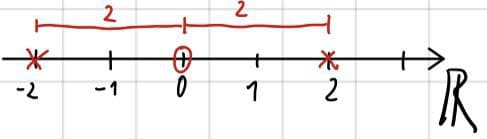
\includegraphics[width=.3\textwidth]{Dateien/05/05Quadrik1.jpg}
\end{center}
\end{Beispiel}
\begin{Beispiel}
{Verschobene Quadrik in 1D (2/7)}
Die Gleichung $\boxed{x^2-2x-8=0}$ können wir durch quadratische Ergänzung in die Form $(x-1)^2=9$ bringen. Die beiden Lösungen können wir uns ebenfalls als 1D-Kugel um den um 1 verschobenen Mittelpunkt vorstellen:
\begin{center}
    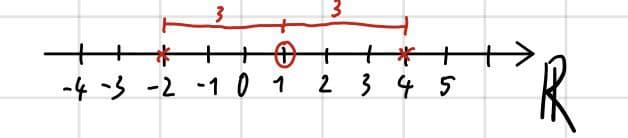
\includegraphics[width=.3\textwidth]{Dateien/05/05Quadrik2.jpg}
\end{center}
\end{Beispiel}

\begin{Beispiel}
{Quadrik in 2D: Kreis (3/7)}
Im Zweidimensionalen ist die einfachste Form einer Quadrik ein Kreis um den Ursprung mit $\boxed{x^2+y^2=16}$.
Wie man sich schnell mit dem Satz des Pythagoras klarmachen kann, sind dies alle Punkte $(x,y)$ mit Abstand $\sqrt{16}=4$ vom Ursprung:
\begin{center}
    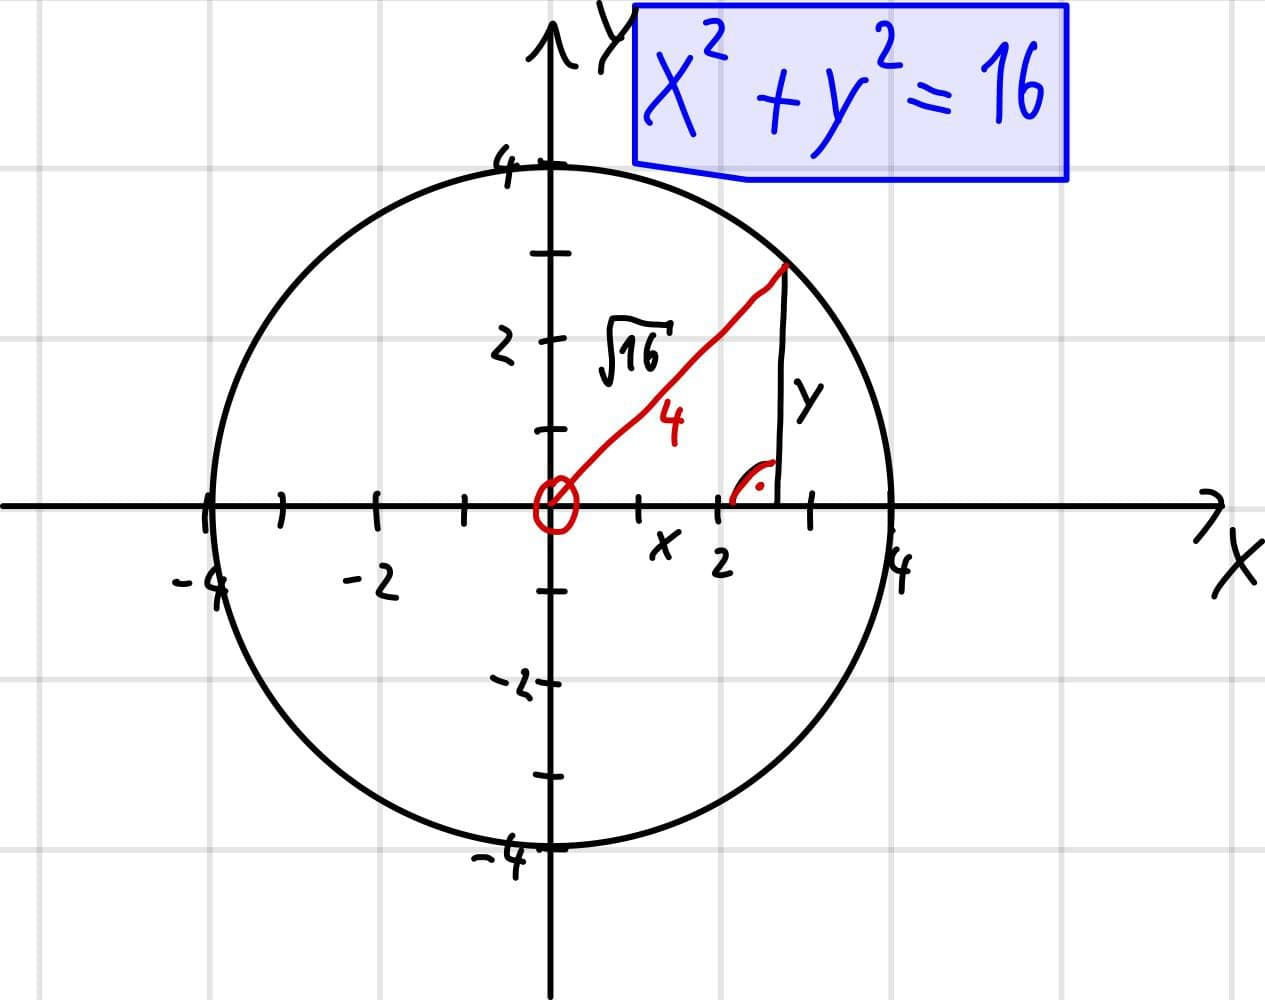
\includegraphics[width=.3\textwidth]{Dateien/05/05Quadrik3.jpg}
\end{center}
Schreiben wir die Bestimmungsgleichung in Matrixform
\begin{equation}
    \vvec^T A \vvec=16\iff \Matrix{x&y}\Matrix{1&0\\0&1}\Matrix{x\\y}=16,
\end{equation}
so sehen wir hier schon, dass diese Matrix eine Signatur von $(2,0,0)$ hat. Dies ist eine Indikation, dass es sich bei der Gleichung um einen Kreis oder eine Ellipse handelt. Die Hauptachsentransformation kann nun auch kompliziertere Gleichungen klassifizieren, wie im übernächsten Beispiel deutlich wird.
\end{Beispiel}

\begin{Beispiel}
{Verschobene Quadrik in 2D: Kreis (4/7)}
Auch diesen Kreis kann man verschieben: $\boxed{x^2+4x+y^2-2x-11=0}$.\\
Mit quadratischer Ergänzung ist dann der Mittelpunkt leicht zu erkennen:\\
$\iff (x+2)^2+(y-1)^2=16$, was dann so aussieht:
\begin{center}
    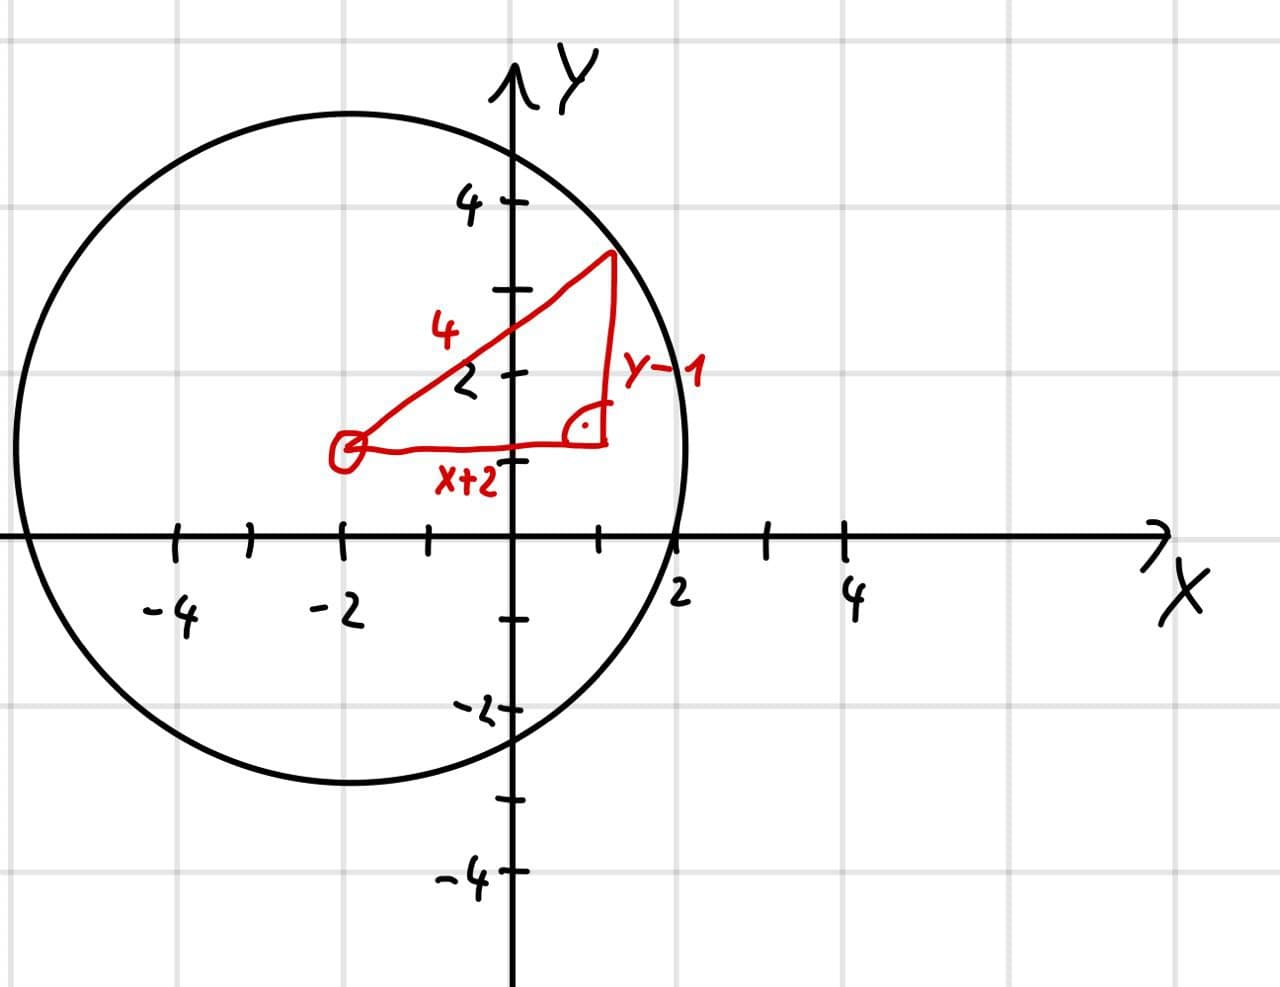
\includegraphics[width=.3\textwidth]{Dateien/05/05Quadrik4.jpg}
\end{center}
\end{Beispiel}

\begin{Beispiel}
{Verschobene Quadrik in 2D: Ellipse (5/7)}
Ähnlich sind Ellipsen zu handhaben.\\
Deren einfachste Form ist $\frac{x^2}{a^2}+\frac{y^2}{b^2}=1$, wobei $a$ und $b$ die \red{Halbachsen} in $x$- und $y$-Richtung sind (auch wieder mit dem Satz des Pythagoras zu sehen). Diese können dann analog zum Kreis verschoben werden.\\
Wir können z. B. $\boxed{\frac{(x-1)^2}{9}+\frac{(y+3)^2}{4}=1}$ (mit dem Mittelpunkt $x=1, y=-3$ und $a=3$ und $b=2$) als Beispiel betrachten:
\begin{center}
    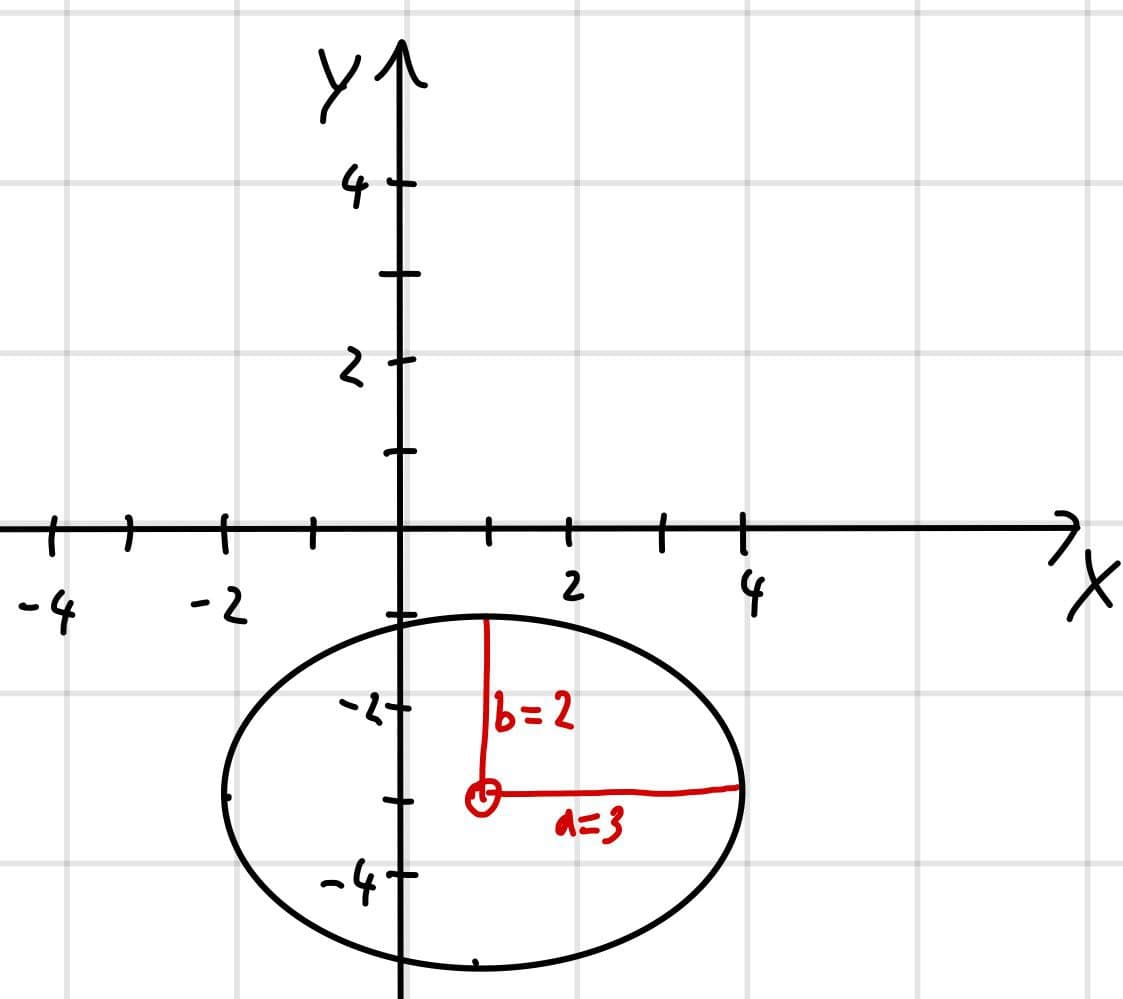
\includegraphics[width=.23\textwidth]{Dateien/05/05Quadrik5.jpg}
\end{center}
\end{Beispiel}
\blue{Wir bekommen bei so etwas allerdings Probleme, sobald Mischterme in unseren Gleichungen auftreten. Diese liefern einen Hinweis darauf, dass die Ellipse gedreht wurde.\\
Um nun die Halbachsen ablesen zu können, müssen wir diese auf die Hauptachse \textit{zurückdrehen}.\\
Hier kommt die Hauptachsentransformation ins Spiel.}
\subsubsection{Drehung einer Quadrik}
\begin{Beispiel}
{Gedrehte Quadrik in 2D: Ellipse und Anwendung der HATrafo (6/7)}
Wir betrachten die Gleichung $\boxed{5x^2-64x+5y^2-32y+6xy+176=0}$ und wollen diese geometrisch interpretieren.\\
Mit $\vvec:=\MatrixInline{x\\y}$ können wir die Gleichung schreiben als
\begin{equation*}
    \Matrix{x & y}\Matrix{5&6/2\\6/2&5}\Matrix{x\\y}+ \Matrix{-64&-32}\Matrix{x\\y}+176=0\iff \vvec^T A \vvec+ \bvec^T\vvec +176 =0,
\end{equation*}
wobei wir $\bvec=-32\MatrixInline{2\\1}$ und $A=\MatrixInline{5&6/2\\6/2&5}$ definieren\footnote{den $xy$-Anteil haben wir hier halbiert, damit die Matrix symmetrisch wird.} bzw. abgelesen haben.\\
Um die Ellipse jetzt \textit{zurückzudrehen}, müssen wir die Eigenwerte $\lambda_i$ und die normierten Eigenvektoren $\wvec_i$ von $A$ finden.
\begin{itemize}
    \item Wir finden 
    \begin{equation*}
        \lambda_1=8\implies \wvec_1=\frac{1}{\sqrt{2}}\Matrix{1\\1},\quad \lambda_2=2\implies \wvec_2=\frac{1}{\sqrt{2}}\Matrix{1\\-1}
    \end{equation*}
    Die diagonalisierte Matrix ist damit
    \begin{equation*}
        D_A=\Matrix{8&0\\0&2},
    \end{equation*}
    was wir testen können, indem wir als $\phi_B$ die Basis der EV bezeichnen:
    \begin{equation*}
        A=\phi_B^{-1} D_A\phi_B=\frac{1}{\sqrt{2}}\Matrix{1&1\\1&-1}\Matrix{8&0\\0&2}\frac{1}{\sqrt{2}}\Matrix{1&1\\1&-1}=\frac{1}{2}\Matrix{10&6\\6&10}=\Matrix{5&3\\3&5}.
    \end{equation*}
    \item Da die Eigenwerte beide positiv sind, ist die Normalform $N_A=\Matrix{1&0\\0&1}$ bzgl. der orthogonalen Basis
\begin{equation*}
    \bvec_1=\frac{\wvec_1}{\sqrt{\Abs{\lambda_1}}\Norm{\wvec_1}}=\frac{1}{\sqrt{8}\sqrt{2}}\Matrix{1\\1}=\frac{1}{4}\Matrix{1\\1},\quad \bvec_2=\frac{1}{2}\Matrix{1\\-1},
\end{equation*}
die Signatur ist also ebenfalls $(2,0,0)$, es handelt sich um eine Ellipse.\footnote{Z. B. beschreiben Gleichungen der Form $(1,1,0)$ Hyperbeln.}
\begin{center}
    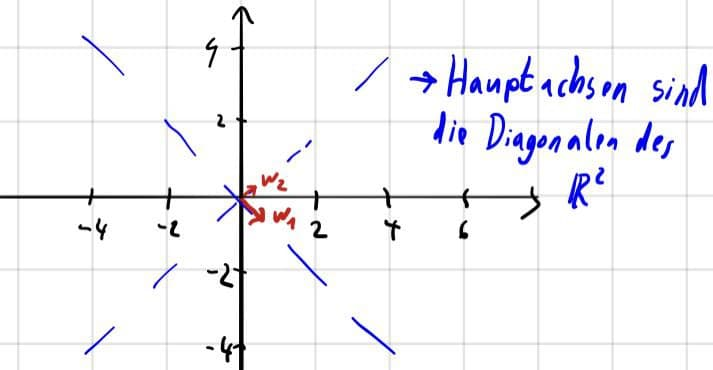
\includegraphics[width=.35\textwidth]{Dateien/05/05DrehungHauptachsen.jpg}
\end{center}
    Damit wir diese Drehung auf die Quadrik anwenden wollen, müssen wir tatsächlich die Normierten Versionen $\bvec_1'=\frac{1}{\sqrt{2}}\MatrixInline{1\\1}$ und $\bvec_2'=\frac{1}{\sqrt{2}}\MatrixInline{1\\-1}$ verwenden, welche in Kombination die Drehmatrix\footnote{also eine lineare Abbildung, bei der die Länge der Vektoren erhalten bleibt, oder auch \textit{orthogonaler Endomorphismus}.} $\mathcal{D}=\frac{1}{\sqrt{2}}\MatrixInline{1&1\\1&-1}$ ergeben, denn
    \begin{equation*}
        \BiFo{\mathcal{D}\vvec,\mathcal{D}\vvec}=(\mathcal{D}\vvec)^T(\mathcal{D}\vvec)=\vvec^T\mathcal{D}^T\mathcal{D} \vvec=\vvec^T\mathds{1}_2\vvec=\BiFo{\vvec,\vvec}.
    \end{equation*}
    Wie oben gesehen, gilt $\mathcal{D}^TA\mathcal{D}=\MatrixInline{8&0\\0&2}$.
    \item Um unsere Gleichung nun in anschauliche Form zu bringen, müssen wir zudem den Vektor $\bvec$ drehen.\\
    Dafür substituieren wir $\vvec=\mathcal{D}\wvec=\mathcal{D}\MatrixInline{x'\\y'}$:
    \begin{eqnarray*}
        0&=&\vvec^T A\vvec-32\bvec^T \vvec+176\\
        \iff0&=&(\mathcal{D}w)^TA \mathcal{D}\wvec-32 \bvec^T\mathcal{D}\wvec+176\\
        \iff 0&=&\wvec^T D_A \wvec+\frac{1}{\sqrt{2}} \bvec^T\Matrix{x'+y'\\x'-y'}+176\\
        \overset{\footnote{Nebenrechnung: $\bvec^T \mathcal{D}\wvec=\MatrixInline{2&1}\MatrixInline{x'+y'\\x'-y'}=2x'+2y'+x'-y'=3x'+y'$}}{\iff} 0&=&8x{'}^2+2y{'}^2-\frac{96}{\sqrt{2}}x'-\frac{32}{\sqrt{2}}y'+176\\
        \overset{\footnote{Nebenrechnung: Zweifache quadratische Ergänzung:\\
        $8(x{'}^2-2\frac{96}{2\cdot 8\sqrt{2}}x'+\frac{6^2}{2}-18)=8(x'-6/\sqrt{2})^2-18\cdot 8$ und\\
        $2(y{'}^2-2\frac{32}{2\cdot 2\sqrt{2}}y'+32-32=2(y'-8/\sqrt{2})^2-32\cdot 2$}}{\iff} 0&=&8\BracedIn{x'-\frac{6}{\sqrt{2}}}^2-144+2\BracedIn{y'-\frac{8}{\sqrt{2}}}^2-64+176\\
        \overset{\footnote{Koordinatentransformation: Wir wählen $x''=x'-\frac{6}{\sqrt{2}}$ und $y''=y'-\frac{8}{\sqrt{2}}$}}{\iff} 32&=&8x{''}^2+2y{''}^2\\
        \iff 1&=&\BracedIn{\frac{x''}{2}}^2+\BracedIn{\frac{y''}{4}}^2.
    \end{eqnarray*}
    Endlich haben wir also unsere bekannte Ellipsenform gefunden!\\
    Es handelt sich also um eine Ellipse mit den Halbachsen $a=2$ und $b=4$, die um $\frac{6}{\sqrt{2}}$ und $\frac{8}{\sqrt{2}}$ verschoben und dann gedreht wurde.
    \item Über eine Rücktransformation kommen wir wieder auf die ursprünglichen Koordinaten:
    \begin{itemize}
        \item Translation: $x''=x'-\frac{6}{\sqrt{2}}$ und $y''=y'-\frac{8}{\sqrt{2}}$ ergibt
        \begin{equation*}
            \BracedIn{\frac{x'-6/\sqrt{2}}{2}}^2+\BracedIn{\frac{y'-8/\sqrt{2}}{4}}^2=1.
        \end{equation*}
        \item Drehung: $\MatrixInline{x\\y}=\mathcal{D}\wvec=\frac{1}{\sqrt{2}}\MatrixInline{x'+y'\\x'-y'}$.\\
        Die Umkehrung davon können wir durch ein Gleichungssystem oder durch Invertieren von $\mathcal{D}$ finden (in diesem Fall gilt $\mathcal{D}^{-1}=\mathcal{D}^T$).\\
        Es zeigt sich, dass $ \MatrixInline{x'\\y'}=\frac{1}{\sqrt{2}}\MatrixInline{x+y\\x-y}$. Somit finden wir:
        \begin{equation*}
            \BracedIn{\frac{x+y-6}{2\sqrt{2}}}^2+\BracedIn{\frac{x-y-8}{4\sqrt{2}}}^2=1.
        \end{equation*}
    \end{itemize}
\end{itemize}
\begin{center}
    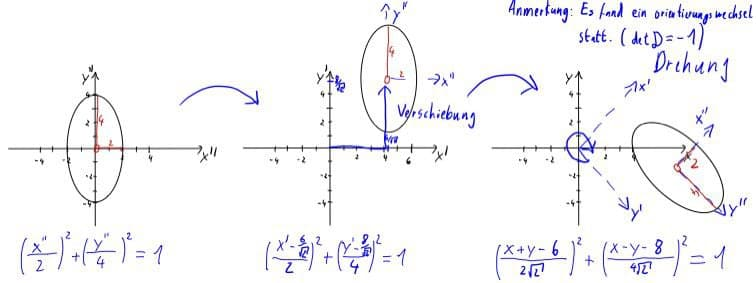
\includegraphics[width=.95\textwidth]{Dateien/05/05DrehungEllipse.jpg}
\end{center}
\end{Beispiel}

\begin{Beispiel}
    {Quadriken in 3D (für Mutige!) (7/7)}
    Wir betrachten die folgende Gleichung:
    \begin{equation*}
        7x^2-2y^2+7z^2+8xy-10xz+8yz+\sqrt{6}x-\sqrt{6}y+1=0.
    \end{equation*}
    Wer jetzt noch nicht die Flucht ergriffen hat, kann sich überlegen, wie man diese Gleichung in Matrizenschreibweise ausdrücken kann. Tatsächlich ist das nämlich gar nicht so übel wie es aussieht. Wir müssen nur vorher die beiden Terme mit der Wurzel abspalten.\\
    Damit erhalten wir:
    \begin{equation*}
        \Matrix{x&y&z}\Matrix{7&4&-5\\4&-2&4\\-5&4&7}\Matrix{x\\y\\z} + \Matrix{\sqrt{6}&-\sqrt{6}&0}\Matrix{x\\y\\z} + 1 = 0.
    \end{equation*}
    Das Ziel dieser Rechnung ist es, herauszufinden, welche geometrische Form diese Gleichung beschreibt.\\
    Dazu wenden wir, wie in den vorherigen Beispielen auch, die Hauptachsentransformation auf die $3\times3$-Matrix an. Da ihr ja mittlerweile Experten seit, rechnen wir die folgenden Schritte nicht ganz so detailliert durch, die Rechnung sollte aber trotzdem gut nachvollziehbar sein.\\
    Fangen wir mit dem charakteristischen Polynom an:
    \begin{equation*}
        0=\det\Matrix{7-\lambda&4&-5\\4&-2-\lambda&4\\-5&4&7-\lambda}=(-6-\lambda)(6-\lambda)(12-\lambda).
    \end{equation*}
    Hier können wir die Eigenwerte $\lambda_1=12$, $\lambda_2=6$ und $\lambda_3=-6$ bequem ablesen. Aus der Diagonalmatrix bekommen wir die Signatur:
    \begin{equation*}
        \Matrix{12&0&0\\0&6&0\\0&0&-6} \qquad \Rightarrow \qquad r_+=2 \quad r_-=1 \quad r_0=0.
    \end{equation*}
    Außerdem können wir die Eigenvektoren bestimmen:
    \begin{align*}
        \lambda_1&=12: \qquad \Matrix{-5&4&-5\\4&-14&4\\-5&4&-5}\Matrix{x\\y\\z}=\Matrix{0\\0\\0} \qquad \Rightarrow \qquad \vvec_1=t\Matrix{1\\0\\-1} \\
        \lambda_2&=6: \qquad \Matrix{1&4&-5\\4&-8&4\\-5&4&1}\Matrix{x\\y\\z}=\Matrix{0\\0\\0} \qquad \Rightarrow \qquad \vvec_2=t\Matrix{1\\1\\1} \\
        \lambda_3&=-6: \qquad \Matrix{13&4&-5\\4&4&4\\-5&4&13}\Matrix{x\\y\\z}=\Matrix{0\\0\\0} \qquad \Rightarrow \qquad \vvec_3=t\Matrix{1\\-2\\1}
    \end{align*}
    und damit die Basis der Normalform anhand der bereits bekannten Formel:
    \begin{align*}
        \wvec_1'&=\frac{\vvec_1}{\lambda_1\Vert \vvec_1\Vert}=\frac{1}{2\sqrt{6}}\Matrix{1\\0\\-1} \\
        \wvec_2'&=\frac{\vvec_2}{\lambda_2\Vert \vvec_2\Vert}=\frac{1}{3\sqrt{2}}\Matrix{1\\1\\1} \\
        \wvec_3'&=\frac{\vvec_3}{\lambda_3\Vert \vvec_3\Vert}=\frac{1}{6}\Matrix{1\\-2\\1}. 
    \end{align*}
    Wenn ihr möchtet, könnt ihr überprüfen, ob diese Vektoren tatsächlich zum richtigen Ergebnis führen.\\
    Sei dazu $F:\mathbb{R}^3 \Rightarrow \mathbb{R}, \, F(\vvec_1,\vvec_2):=\vvec_1^T A \vvec_2$ mit einer $3\times3$-Matrix $A$, dann erhalten wir:
    \begin{equation*}
        A:=\Matrix{7&4&-5\\4&-2&4\\-5&4&7} \qquad \Rightarrow \qquad (F(\wvec_i',\wvec_j'))_{ij}=\Matrix{1&0&0\\0&1&0\\0&0&-1}
    \end{equation*}
    Nun folgt die eigentliche Anwendung auf die Quadrik. Diese dürfen wir nur drehen und verschieben, da ja die Form beibehalten werden soll (um später identifizieren zu können, um welchen Kegelschnitt es sich handelt). \\
    Der erste Schritt dafür ist, die Vektoren $\wvec_1'$, $\wvec_2'$ und $\wvec_3'$ zu orthonormalisieren:
    \begin{align*}
        \wvec_1&=\frac{\wvec_1'}{\Vert \wvec_1' \Vert} = \frac{1}{\sqrt{2}}\Matrix{1\\0\\-1} \\
        \wvec_2&=\frac{\wvec_2'}{\Vert \wvec_2' \Vert} = \frac{1}{\sqrt{3}}\Matrix{1\\1\\1} \\
        \wvec_3&=\frac{\wvec_3'}{\Vert \wvec_3' \Vert} = \frac{1}{\sqrt{6}}\Matrix{1\\-2\\1}.
    \end{align*}
    Wir können uns auch hier wieder überzeugen, dass nun:
    \begin{equation*}
        (F(\wvec_i,\wvec_j))_{ij}=\Matrix{12&0&0\\0&6&0\\0&0&-6}.
    \end{equation*}
    Nun beginnt die eigentliche Zauberei der Hauptachsentransformation.\\
    Wenn ihr bis hierhin gut aufgepasst habt, wisst ihr, dass man die Matrix $A$ in ihre Diagonalform transformieren kann, wenn man die orthonormierten Basisvektoren als Spalten in eine Matrix $B$ schreibt:
    \begin{equation*}
        B:=\Matrix{\frac{1}{\sqrt{2}}&\frac{1}{\sqrt{3}}&\frac{1}{\sqrt{6}}\\0&\frac{1}{\sqrt{3}}&-\frac{2}{\sqrt{6}}\\-\frac{1}{\sqrt{2}}&\frac{1}{\sqrt{3}}&\frac{1}{\sqrt{6}}}.
    \end{equation*}
    Diese Matrix ist eine Drehmatrix! Dies kann man sich durch
    \begin{equation*}
        \langle Bv, Bw \rangle = \sum_{i,j=1}^{3}x_ix_j\langle \wvec_i, \wvec_j \rangle = \sum_{i,j=1}^{3} x_i y_j \delta_{ij} = \sum_{i=1}^{3} x_i y_i = \langle x,y \rangle
    \end{equation*}
    deutlich machen, da die Vektoren $\wvec_i$ orthogonal aufeinander stehen. \\
    Sei nun $\vvec=(x,y,z)^T$. In unsere ursprüngliche Gleichung setzen wir nun $\vvec=B\uvec$ mit einem beliebigen Vektor $\uvec$:
    \begin{align*}
        \uvec^T B^T \Matrix{7&4&-5\\4&-2&4\\-5&4&7}B\uvec + \Matrix{\sqrt{6}&-\sqrt{6} 0}B\uvec + 1 = 0 \\
        \Rightarrow \uvec^T\Matrix{12&0&0\\0&6&0\\0&0&-6}\uvec + \Matrix{\sqrt{3}&0&3}\uvec + 1 = 0
    \end{align*}
    Damit sind die Mischterme (also $axy$, $byz$ usw.) in der ursprünglichen Gleichung erfolgreich eliminiert (nice!).\\
    Alles Weitere ist nun geschicktes Umformen.\\
    Wir definieren dazu unser Koordinatensystem um und setzen $\uvec=\Matrix{x&y&z}^T$:
    \begin{align*}
        &12x^2+6y^2-6z^2+\sqrt{3}x+3z+1=0 \\
        \Leftrightarrow &12(x+\frac{\sqrt{3}}{24})^2-\frac{3}{48}+6y^2-6(z-\frac{1}{4})^2+\frac{3}{8} + 1 = 0 \\
        \Leftrightarrow &12(x+\frac{\sqrt{3}}{24})^2 + 6y^2 - 6(z-\frac{1}{4})^2 = -\frac{21}{16}.
    \end{align*}
    Nun führen wir eine Translation durch, indem wir $x$, $y$ und $z$ erneut umdefinieren:
    \begin{equation*}
        x \longrightarrow x-\frac{\sqrt{3}}{24} \qquad y \longrightarrow y \qquad z \longrightarrow z+\frac{1}{4}
    \end{equation*}
    Dadurch erhalten wir
    \begin{align*}
        12x^2+6y^2-6z^2=-\frac{21}{16} \\
        \Leftrightarrow -\frac{x^2}{\alpha_1^2}-\frac{y^2}{\alpha_2^2}+\frac{z^2}{\alpha_3^2}=1,
    \end{align*}
    wobei wir im letzten Schritt die folgenden Abkürzungen verwendet haben:
    \begin{equation*}
        \alpha_1 = \sqrt{\frac{7}{64}} \qquad \alpha_2 = \sqrt{\frac{7}{32}} \qquad \alpha_3 = \sqrt{\frac{7}{32}}
    \end{equation*}
    Diese nun sehr kompakte Gleichung beschreibt dieselbe Form wie vorher, wir haben sie nur etwas gedreht und verschoben\footnote{bzw. haben wir das \textit{Koordinatensystem} gedreht und verschoben.}. Der Vorteil an dieser kompakten Form ist nun, dass wir ganz leicht die Art des Kegelschnittes ablesen können (etwas Übung vorausgesetzt natürlich).\\
    In diesem Fall handelt es sich um ein \red{zweischaliges Hyperboloid}. \\
    Die abschließende Abbildung hilft hoffentlich dabei, sich den Vorgang auch in 3D bildlich vorstellen zu können.
    \begin{center}
        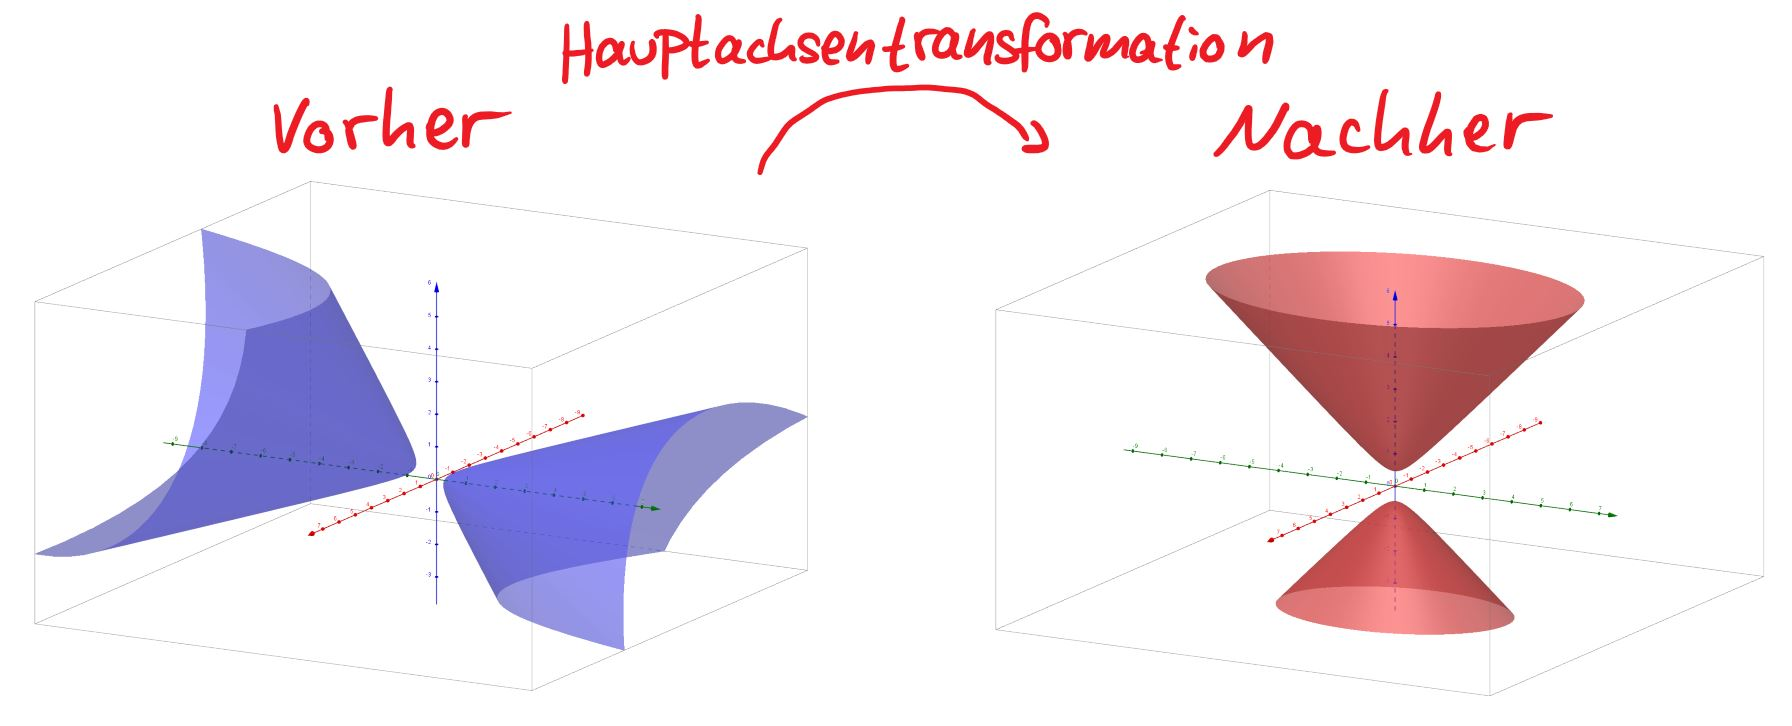
\includegraphics[width=.95\textwidth]{Dateien/05/05Quadrik6.JPG}
    \end{center}
\end{Beispiel}

\subsection{Vollständige metrische Räume}
\blue{Lasst uns nun zum nächsten Thema kommen: Vollständige metrische Räume und der banachsche Fixpunktsatz. Dazu müssen wir uns zunächst durch ein paar Definitionen und Wiederholungen kämpfen.}
\begin{Wiederholung}
{Metrik}
Eine Abstandsfunktion oder \red{Metrik $d$} ordnet zwei Elementen einer Menge $X$ eine positive reelle Zahl zu und hat die folgenden Eigenschaften:\\
$d:X\times X\to [0,\infty)$
\begin{eqnarray*}
\red{M1}: & d(x,y)\geq 0\text{ und } d(x,y)=0\Leftrightarrow x= y &\red{'positiv definit'}\\
\red{M2}: & d(x,y)=d(y, x) &\red{'symmetrisch'}\\
\red{M3}: & d(x,y)\leq d(x, z)+d(y,z) & \red{'Dreiecksungleichung'}.
\end{eqnarray*}
\end{Wiederholung}
\begin{Def}
{Metrischer Raum}
Wir nennen eine Menge $X$ zusammen mit einer Metrik einen \red{metrischen Raum}.
\end{Def}
\begin{Beispiel}
{Die reellen Zahlen als metrischer Raum}
Mit dem der Differenz des Betrages als Abstandsfunktion\\ ($d:\mathbb{R}\times\mathbb{R}\to[0,\infty)\,d(x,y):=\Abs{x-y}$) sind die reellen Zahlen ein metrischer Raum, wie wir in Mathe 1 gesehen hatten.
\end{Beispiel}

\begin{Def}
{Norm}
Falls wir Vektorräume $V$ über $\mathbb{K}$ betrachten, können wir dort noch den Begriff der \red{Norm} spezifizieren, der jedem Vektor $\vvec\in V$ eine Länge zuordnet:
\begin{equation}
    \Norm{\cdot}:V\to[0,\infty),\quad \vvec\mapsto\Norm{\vvec}.
\end{equation}
Zudem müssen die drei \textit{Normaxiome} N1, N2 und N3 erfüllt sein:
\begin{itemize}
    \item N1: \red{Positive Definitheit}: $\Norm{\vvec}=0\iff \vvec=0$ für $\vvec\in V$.
    \item N2: \red{Homogenität (Skalierung)}: $\Norm{\lambda \vvec}=\Abs{\lambda}\Norm{\vvec}$ für alle $\vvec\in V,\lambda \in\mathbb{K}$.
    \item N3: \red{Dreiecksungleichung}: $\Norm{\vvec+\wvec}\leq\Norm{\vvec}+\Norm{\wvec}$ für alle $\vvec,\wvec\in V$ \blue{(i. d. R. am schwierigsten zu zeigen).}
\end{itemize}
\end{Def}
\red{Achtung: Bisher hatten wir nur Normen kennengelernt, die durch ein Skalarprodukt \textit{induziert} wurden ($\Norm{\vvec}=\sqrt{\BiFo{\vvec,\vvec}}$). Dies muss aber nicht unbedingt der Fall sein!}
\begin{Beispiel}
{Die Maximumsnorm auf dem $\mathbb{R}^n$}
\Zz{Durch $\Norm{\xvec}_\tx{max}:=\max(\Abs{x_1},\Abs{x_2},\ldots,\Abs{x_n})$ ist auf $V=\mathbb{R}^n$ eine Norm definiert.}
Anwendungsbeispiel: Sei $\vvec=\MatrixInline{1\\-8\\2}\in\mathbb{R}^3\implies\Norm{\vvec}_\tx{max}=\max(1,8,2)=8$.\\
\Zb{Wir zeigen, dass $\Norm{\cdot}_{\max}$ die Normaxiome erfüllt.
\begin{itemize}
    \item N1)
    \begin{itemize}
        \item \grqq$\implies$\grqq: Für $\Norm{\xvec}_{\max}=0$ muss $\xvec$ der Nullvektor sein, denn wäre O.B.D.A.\footnote{Ohne Beschränkung der Allgemeinheit} der erste Eintrag ungleich 0, so wäre $\Norm{\xvec}_{\max}=\max(\Abs{x_1},0,\ldots,0)=\Abs{x_1}\neq0$, was im Widerspruch zur Annahme steht.
        \item \grqq$\impliedby$\grqq: Ist $\xvec=0$, so ist $\Norm{\xvec}_{\max}=\max(0,\ldots,0)=0.\,\checkmark$
    \end{itemize}
    \item N2) $\forall\lambda\in\mathbb{R},\,\,\xvec\in\mathbb{R}^n$ gilt:
    \begin{align*}
        \Norm{\lambda \xvec}_\tx{max}&=\max(\Abs{\lambda x_1},\Abs{\lambda x_2},\ldots,\Abs{\lambda x_n})\\
        &=\max(\Abs{\lambda}\Abs{ x_1},\Abs{\lambda}\Abs{ x_2},\ldots,\Abs{\lambda}\Abs{ x_n})\\
        &=\Abs{\lambda}\max(\Abs{x_1},\ldots,\Abs{x_n})=\Abs{\lambda}\Norm{\xvec}_\tx{max}.\,\checkmark
    \end{align*}
    \item N3) Wir müssen zeigen: $\Norm{\xvec+\yvec}_\tx{max}\leq\Norm{\xvec}_\tx{max}+\Norm{\yvec}_\tx{max}\,\forall \xvec,\yvec\in\mathbb{R}^n$:
    \begin{eqnarray*}
        \Norm{\xvec+\yvec}_\tx{max}&=&\max(\Abs{x_1+y_1},\ldots,\Abs{x_n+y_n})\\
        &\overset{\footnote{Wir nutzen die Dreiecksungleichung für den Betrag für jede Komponente.}}{\leq}&\max(\Abs{x_1}+\Abs{y_1},\ldots,\Abs{x_n}+\Abs{y_n})\\
        &\overset{\footnote{Wir nutzen $\max(\Abs{a}+\Abs{b})=\Abs{a}+\Abs{b}\leq\max(\Abs{a})+\max(\Abs{b})$}}{\leq}&\max(\Abs{x_1},\ldots,\Abs{x_n})+\max(\Abs{y_1},\ldots,\Abs{y_n})\\
        &=&\Norm{\xvec}_\tx{max}+\Norm{\yvec}_\tx{max}.\,\checkmark
    \end{eqnarray*}
\end{itemize}
}
\end{Beispiel}
\begin{Satz}
{Anmerkung}{Vom Skalarprodukt induzierte Norm}
In euklidischen/hermiteschen Vektorräumen $(V,\BiFo{\cdot,\cdot})$ ist stets die vom Skalarprodukt induzierte Norm durch $\Norm{\vvec}=\sqrt{\BiFo{\vvec,\vvec}}$ auf $V$ definiert.\\
Diese erfüllt die Normaxiome, denn:
\begin{itemize}
    \item N1) folgt aus der positiven Definitheit des Skalarproduktes.
    \item N2) Es ist $\Norm{\lambda \vvec}^2=\BiFo{\lambda \vvec,\lambda \vvec}\overset{\footnote{$(\mathbb{C})$-Linearität}}{=}\Abs{\lambda}^2\BiFo{\vvec,\vvec}=\Abs{\lambda}^2\Norm{\vvec}^2$.
    \item N3) Es ist
    \begin{eqnarray*}
    \Norm{\vvec+\wvec}^2&=&\BiFo{\vvec+\wvec,\vvec+\wvec}\overset{\footnote{Bilinearität}}{=}\BiFo{\vvec,\vvec}+\BiFo{\vvec,\wvec}+\BiFo{\wvec,\vvec}+\BiFo{\wvec,\wvec}\\
    &\overset{\footnote{Hermitizität, $\frac{1}{2}(\BiFo{\vvec,\wvec}+\overline{\BiFo{\vvec,\wvec}})=\Re(\BiFo{\vvec,\wvec})$}}{=}&\Norm{\vvec}^2+\Norm{\wvec}^2+2\Re(\BiFo{\vvec,\wvec})\overset{\footnote{Gleichheit gilt, wenn $\Re(\BiFo{\vvec,\wvec})=\Abs{\BiFo{\vvec,\wvec}}$}}{=}\Norm{\vvec}^2+\Norm{\wvec}^2+2\Abs{\BiFo{\vvec,\wvec}}\\
    &\overset{\footnote{Cauchy-Schwarzsche Ungleichung}}{\leq}&\Abs{\vvec}^2+\Abs{\wvec}^2+2\Norm{\vvec}\Norm{\wvec}\overset{\footnote{Binomische Formeln}}{=}(\Norm{\vvec}+\Norm{\wvec})^2.
    \end{eqnarray*}
\end{itemize}
\end{Satz}
\blue{Mithilfe der folgenden Gleichung können wir überprüfen, ob eine vorgegebene Norm durch ein Skalarprodukt induziert wurde:}
\begin{Satz}
{Satz}{Parallelogrammgleichung}
Genau dann wenn eine Norm $\Norm{\cdot}$ auf einem Vektorraum $V$ über $\mathbb{R}$ durch ein Skalarprodukt induziert wird, gilt die \red{Parallelogrammgleichung}
\begin{equation*}
    \Norm{\vvec+\wvec}^2+\Norm{\vvec-\wvec}^2=2\Norm{\vvec}^2+2\Norm{\wvec}^2\quad \forall \vvec,\wvec\in V.
\end{equation*}
\begin{center}
    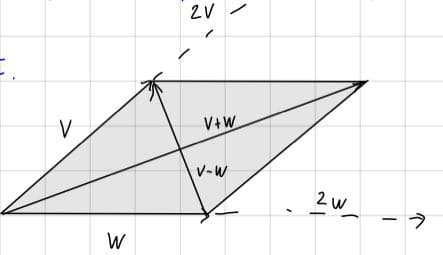
\includegraphics[width=.5\textwidth]{Dateien/05/05Parallelogramm.jpg}
\end{center}
\end{Satz}
\begin{Beispiel}
{Beweis in die eine Richtung}
Wir zeigen kurz, dass dies mit einer vom Skalarprodukt induzierten Norm klappt:
\begin{align*}
    \Norm{\vvec+\wvec}^2+\Norm{\vvec-\wvec}^2&=\BiFo{\vvec+\wvec,\vvec+\wvec}+\BiFo{\vvec-\wvec,\vvec-\wvec}\\
    &=\BiFo{\vvec,\vvec}+2\Re(\BiFo{\vvec,\wvec})+\BiFo{\wvec,\wvec}+\BiFo{\vvec,\vvec}-2\Re(\BiFo{\vvec,\wvec})+\BiFo{\wvec,\wvec}\\
    &=2\BiFo{\vvec,\vvec}+2\BiFo{\wvec,\wvec}.
\end{align*}
Die andere Richtung ist aufwändiger, siehe \Skript{}.
\end{Beispiel}

\begin{Satz}
{Anmerkung}{Verknüpfung der Norm zur Metrik}
Jede Norm definiert durch $d:V\times V\to [0,\infty),\,d(\xvec,\yvec)=\Norm{\xvec-\yvec}$ auch eine Metrik auf $V$, denn die Metrikaxiome M1), M2) und M3) folgen aus den Eigenschaften der Norm:
\begin{itemize}
    \item M2): $d(\xvec,\yvec)=\Norm{\xvec-\yvec}=\Norm{(-1)(\yvec-\xvec)}\overset{\tx{N2)}}{=}\Abs{-1}\Norm{\yvec-\xvec}=\Norm{\yvec-\xvec}=d(\yvec,\xvec)$.
    \item M3): $d(\xvec,\zvec)=\Norm{\xvec-\zvec}=\Norm{\xvec+\yvec-\yvec-\zvec}\overset{\tx{N3)}}{\leq}\Norm{\xvec-\yvec}+\Norm{\yvec-\zvec}=d(\xvec,\yvec)+d(\yvec,\zvec)$.
\end{itemize}
\end{Satz}
\subsubsection{Offene Kugel für verschiedene Metriken}
Wir machen nun einen Vorgriff auf eine kommende Definition, um Unterschiede zwischen verschiedenen Metriken zu verdeutlichen:
\begin{Def}
{Offene Kugel}
Die Teilmenge $\boxed{B_r(\xvec):=\Menge{\yvec\in X}{d(\xvec,\yvec)<r}\subseteq X}$ eines metrischen Raumes $(X,d)$ mit Abstandsfunktion $d$ heißt \red{offene Kugel} mit Mittelpunkt $\xvec$ und Radius $r$.
\end{Def}
\blue{Diese Definition können wir uns z. B. im $\mathbb{R}^3$ mit der euklidischen Metrik tatsächlich als herkömmliche Kugel vorstellen.\\
Aber Achtung: Je nach Metrik kann eine solche 'offene Kugel' anders aussehen!}\\
Für die folgenden Beispiele betrachten wir $B_1(0)$ im $\mathbb{R}^2$ (also eine Kugel um 0 mit Radius 1).
\begin{Beispiel}{Euklidische Metrik (1/3)}
Mit der euklidischen Metrik $d_2(\xvec,\yvec)=\sqrt{\sum_{i=1}^2\Abs{x_i-y_i}^2}$ ist die offene Kugel einfach ein Kreis.\\ $B_1(0)$ sieht also so aus:
\begin{center}
    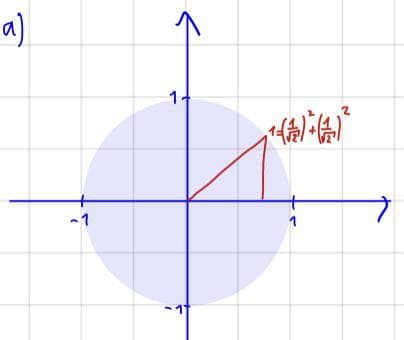
\includegraphics[width=.35\textwidth]{Dateien/05/05Metrik1.jpg}
\end{center}
\end{Beispiel}
\begin{Beispiel}
{Summenmetrik (2/3)}
Mit der Summenmetrik $d_1(\xvec,\yvec):=\sum_{i=1}^2\Abs{x_i-y_i}$ ist die offene Kugel hingegen ein gedrehtes Quadrat, dessen Kantenlänge in diesem Fall $\sqrt{2}$ ist.\\ Hier sieht $B_1(0)$ so aus:
\begin{center}
    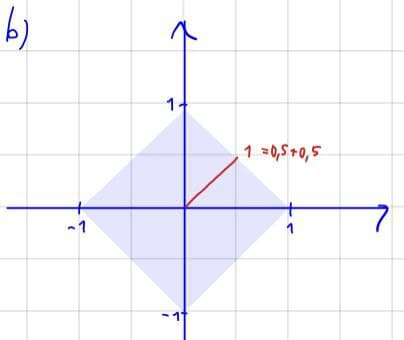
\includegraphics[width=.35\textwidth]{Dateien/05/05Metrik2.jpg}
\end{center}
\end{Beispiel}
\begin{Beispiel}
{Maximumsmetrik (3/3)}
Mit der Maximumsmetrik $d_\tx{max}(\xvec,\yvec):=\max(\Abs{x_1-y_1},\Abs{x_2-y_2})$ ist die offene Kugel ein Quadrat mit Kantenlänge 2.\\ Hier sieht $B_1(0)$ so aus:
\begin{center}
    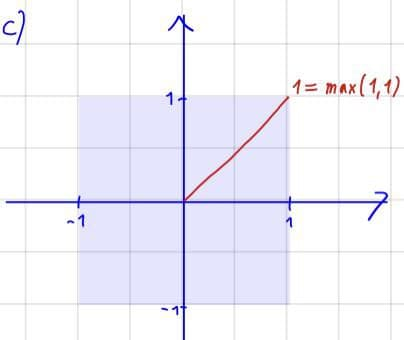
\includegraphics[width=.35\textwidth]{Dateien/05/05Metrik3.jpg}
\end{center}
\end{Beispiel}

\begin{Def}
{Äquivalente Normen}
Wir nennen zwei Normen $\Norm{\cdot}_1$ und $\Norm{\cdot}_2$ auf einem Vektorraum \red{äquivalent}, falls es Schranken $c,C\in\mathbb{R}$ gibt, sodass
\begin{equation}
    c\Norm{\vvec}_1\leq\Norm{\vvec}_2\leq C\Norm{\vvec}_1\quad \forall v\in V.
\end{equation}
\end{Def}
\blue{Wir müssen mit der einen Norm also quasi die andere einschränken können, falls sie äquivalent sind.}
\begin{Beispiel}
{Beweis: Die Äquivalenz zwischen Normen ist eine Äquivalenzrelation}
Wir beweisen die obige Aussage.\\
\Zb{Die Normäquivalenz definiert eine Äquivalenzrelation, denn:
\begin{itemize}
    \item Sie ist reflexiv:\\
    Eine beliebige Norm ist mit den Konstanten $c=C=1$ stets zu sich selbst äquivalent.
    \item Sie ist symmetrisch:\\
    Sei $\Norm{\cdot}_1$ zu $\Norm{\cdot}_2$ äquivalent, es gebe also $c,C$ sodass $c\Norm{\vvec}_1\leq\Norm{\vvec}_2\leq C\Norm{\vvec}_1$.\\
    Dann ist aber $\frac{1}{C}\Norm{\vvec}_2\leq\Norm{\vvec}_1\leq\frac{1}{c}\Norm{\vvec}_2$, $\Norm{\cdot}_2$ ist also äquivalent zu $\Norm{\cdot}_1$.
    \item Sie ist transitiv:\\
    Seien $\Norm{\cdot}_1\sim \Norm{\cdot}_2$ und $\Norm{\cdot}_1\sim\Norm{\cdot}_3$, dann ist
    \begin{align*}
        &c\Norm{\vvec}_1\leq\Norm{\vvec}_2\leq C\Norm{\vvec}_1\,\land\, c'\Norm{\vvec}_1\leq\Norm{\vvec}_3\leq C'\Norm{\vvec}_1\\
        \implies & c\Norm{\vvec}_1\leq\frac{c}{c'}\Norm{\vvec}_3\leq\Norm{\vvec}_2\leq\frac{C}{C'}\Norm{\vvec}_3\leq C\Norm{\vvec}_1,
    \end{align*}
    also ist $\Norm{\cdot}_1\sim\Norm{\cdot}_2$.
\end{itemize}}
\end{Beispiel}
\begin{Beispiel}
{Die Maximumsnorm und die Betragssummennorm sind äquivalent}
\Zz{Die Maximumsnorm $\Norm{\xvec}_\tx{max}=\max(\Abs{x_1},\ldots,\Abs{x_n})$ und die Betragssummennorm $\Norm{\xvec}_1=\sum_{i=1}^n\Abs{x_i}$ auf dem $\mathbb{R}^n$ sind äquivalent.}
\Zb{Es gilt:
\begin{equation*}
    \Abs{x_i}\leq\max(\Abs{x_1},\ldots,\Abs{x_n})\,\forall i\overset{\footnote{Wenn wir das für die Summe über alle $i$ machen, finden wir $\sum_{i=1}^n\Abs{x_i}\leq n\max(\Abs{x_1},\ldots,\Abs{x_n})$}}{\implies} \Norm{\xvec}_1\leq n\Norm{\xvec}_\tx{max}.
\end{equation*}}\\
Außerdem gilt
\begin{equation*}
    \Norm{\xvec}_\tx{max}=\max(\Abs{x_1},\ldots,\Abs{x_n})\leq\sum_{i=1}^n\Abs{x_i}=\Norm{\xvec}_1.
\end{equation*}
Mit $c:=1$ und $C:=n$ gilt also $c\Norm{\xvec}_\tx{max}\leq\Norm{\xvec}_1\leq\Norm{\xvec}_\tx{max}$, d. h. $\Norm{\cdot}_1\sim\Norm{\cdot}_\tx{max}$.
\end{Beispiel}
Dass diese beiden Normen auf dem endlichdimensionalen $\mathbb{R}^n$ äquivalent sind, ist kein Wunder, denn:
\begin{Satz}
{Satz}{Äquivalenz von Normen auf endlichdimensionalen Vektorräumen}
Auf endlichdimensionalen Vektorräumen sind zwei beliebige Normen immer äquivalent.
\end{Satz}

\subsection{Kontrahierende Abbildungen und der Banachsche Fixpunktsatz}
\begin{Def}
{Kontrahierende Abbildung}
Wir nennen eine Abbildung $F:X\to X$ auf einem metrischen Raum $(X,d)$ \red{kontrahierend}, wenn $\forall x,y\in X$ gilt:
\begin{equation*}
    d(F(x),F(y))\leq \theta d(x,y)\quad\tx{mit }0\leq\theta <1.
\end{equation*}
\end{Def}
\blue{Das Kriterium können wir (für $d(x,y)\neq0$) auch umschreiben zu
\begin{equation*}
    \frac{d(F(x),F(y))}{d(x,y)}<1,
\end{equation*}
die Funktionswerte liegen also immer näher zusammen als deren Urbilder.}
\begin{Beispiel}
{Kontrahierende Gerade (1/2)}
Die Gerade $g:\mathbb{R}\to\mathbb{R},\,g(x)=2-0.5x$ (wobei $d:\mathbb{R}\times\mathbb{R}\to\mathbb{R}$ die Betragsmetrik sei) ist kontrahierend, denn
\begin{equation*}
    d(g(x),g(y))=\Abs{2-0.5x-(2-0.5y)}=\Abs{-0.5}\Abs{x-y}=0.5\Abs{x-y}=\theta d(x,y).
\end{equation*}
\end{Beispiel}

\begin{Wiederholung}{Mittelwertsatz}
Ist $f:[a,b]\to\mathbb{R}$ stetig und differenzierbar auf $(a,b)$, so existiert ein\\
$\xi\in(a,b)$, sodass $f'(\xi)=\frac{f(b)-f(a)}{b-a}$.
\end{Wiederholung}
\begin{Beispiel}
{Verknüpfung mit dem Mittelwertsatz (1/2)}
Für Funktionen $f:\mathbb{R}\to\mathbb{R}$ mit der Betragsmetrik können wir $\theta$ explizit berechnen:\\
Für gegebene $x,y\in\mathbb{R}$ wissen wir aufgrund des Mittelwertsatzes, dass $\xi\in[x,y]$ existiert, sodass
\begin{equation*}
    \theta=\Abs{f'(\xi)}=\frac{\Abs{f(x)-f(y)}}{\Abs{x-y}}.
\end{equation*}
Nach einer Abschätzung für ganze Intervalle können wir das auf den gesamten Definitionsbereich verallgemeinern.\\
Als Beispiel betrachten wir $F:[1,\infty)\to\mathbb{R},\,x\mapsto \frac{1}{2}x+\frac{1}{x}$.\\
Dann ist $\frac{\Abs{F(x)-F(y)}}{\Abs{x-y}}=\Abs{F'(\xi)}=\Abs{\frac{1}{2}-\frac{1}{\xi^2}}\overset{\footnote{weil $\xi\in[1,\infty)$ ist $\Abs{1/\xi^2}\leq 1$}}{\leq}\frac{1}{2}=:\theta\,\forall x,y\in [1,\infty)$. $F$ ist somit eine kontrahierende Abbildung. 
\end{Beispiel}
Diesen Begriff benötigen wir für den folgenden, erstaunlichen Satz:
\begin{Satz}
{Satz}{Banachscher Fixpunktsatz}
Für jede kontrahierende Abbildung in einem \underline{vollständigen}\footnote{Wdh.: In einem vollständigen Raum konvergiert jede Cauchy-Folge gegen ein Element aus diesem Raum.} metrischen Raum $(X,d)$ existiert ein \underline{eindeutiger} \red{Fixpunkt} $\Tilde{x}\in X$, für den gilt, dass $\boxed{F(\Tilde{x})=\Tilde{x}}$.\\
Zudem konvergiert die Folge $\boxed{x_{k+1}=F(x_k)}$ für alle Anfangswerte $x_0\in X$ gegen den Fixpunkt, $\lim_{n\to\infty}x_n=\Tilde{x}$.
\end{Satz}
\blue{\textbf{Motivation/Anwendung}:\\
Wir werden sehen, dass die Eindeutigkeit dieses Fixpunkts wahnsinnig nützlich werden kann, wenn wir uns gegen Ende des Semesters Differentialgleichungen (DG) anschauen. Dort wird eine der wichtigsten Aussagen sein, dass eine DG der Form $x'=F(x,t)$ mit $x(t_0)=x_0$ \underline{genau eine} Lösung hat, wenn $F$ bestimmte Bedingungen erfüllt.\\
Für den Beweis wird dort der Raum der stetigen Funktionen mit einer Norm verwendet, auf dem ein Integraloperator\footnote{der dann auch noch genauer definiert wird und im Prinzip $F(x,t)$ über $t$ integriert.} stetige Funktionen auf stetige Funktionen abbildet. Diese Abbildung ist kontrahierend und besitzt demnach einen Fixpunkt, der \underline{eindeutige} Lösung. Das Iterationsverfahren aus dem Fixpunktsatz kann dann mit diesem Integraloperator auch zum Finden der Lösung der Differentialgleichung verwendet werden.}
\begin{Beispiel}
{Umgebungskarte (1/3)}
Wenn man eine verkleinerte Karte der Umgebung betrachtet, so existiert genau ein Punkt auf der Karte, der dem Ort entspricht, wo die Karte sich befindet.
\end{Beispiel}

\begin{Beispiel}
{Fixpunkt der Geradenabbildung (2/3)}
Wir hatten gesehen, dass $g:\mathbb{R}\to\mathbb{R},\,g(x)=2-0.5x$ kontrahierend mit $\theta=0.5$ ist.\\
Um den Fixpunkt zu finden, lösen wir die Gleichung
\begin{align*}
    \Tilde{x}=2-0.5\Tilde{x}\iff \frac{3}{2}\Tilde{x}=2\iff \Tilde{x}=\frac{4}{3}.
\end{align*}
Alternativ könnt ihr euch auch daran versuchen, eine explizite Vorschrift für die Folge $x_{k+1}=2-0.5x_k$ zu finden, diese zu beweisen und abschließend noch zu zeigen, dass diese gegen $\frac{4}{3}$ konvergiert. Schreibt uns gern, vielleicht bauen wir das in zukünftige Versionen ein, Stand jetzt hatten wir keine Zeit,\footnote{wobei ihr euch wahrscheinlich fragen werdet, warum gerade \textit{das} nun den Rahmen sprengt :D} uns damit zu befassen.
\end{Beispiel}

\begin{Beispiel}
{Fixpunkt einer weiteren Funktion (3/3)}
Wir hatten oben gesehen, dass $F:[0,\infty)\to[0,\infty),\,x\mapsto \frac{1}{2}x+\frac{1}{x}$ eine kontrahierende Abbildung ist. Der Fixpunkt ist dann gegeben durch
\begin{equation*}
    \Tilde{x}=\frac{\Tilde{x}}{2}+\frac{1}{\Tilde{x}}\iff \frac{1}{2}\Tilde{x}^2=1\overset{\footnote{$-\sqrt{2}$ ist nicht Teil des Definitionsbereiches.}}{\implies} \Tilde{x}=\sqrt{2}.
\end{equation*}
Die Folge $x_{n+1}=F(x_n)=\frac{1}{2}\BracedIn{x_n+\frac{2}{x_n}}$ war in MfP1 genau jene Folge, die ihr genutzt hattet, um zu zeigen, dass die rationalen Zahlen nicht vollständig sind!
\end{Beispiel}

\Tipps{7}{
\begin{enumerate}
    \item Die Signaturbestimmung sollte euch leicht fallen (vergleicht sonst mit Beispielen in unseren Notizen zu letzter Woche).\\
    Für b) müsst ihr euch ein bisschen mehr überlegen. Vielleicht hilft hier ebenfalls ein Blick in unsere Notizen zu letzter Woche.
    \item Diese Aufgabe ist dazu da, euch mit den Normaxiomen vertraut zu machen. Denkt daran, auch zu argumentieren, weshalb der Bildbereich einer Norm getroffen wird. Dazu haben wir auch ein paar sicherlich hilfreiche Beispiele betrachtet. Zur Äquivalenz gibt es einen Satz über Normen auf bestimmten Vektorräumen - was könnte hier also schief gehen?
    \item Für diese Aufgaben ist genaues Nachschlagen der Definitionen (was war nochmal Abgeschlossenheit, wie können wir die Euklidische Metrik nutzen usw.) erforderlich.
    \item
    \begin{enumerate}
        \item Die Operatornorm $\Norm{\cdot}_\tx{op}$ sieht gruseliger aus, als sie ist. Im Allgemeinen ist zu beachten, dass sie für Abbildungen $F:V_1\to V_2$ zwischen normierten Vektorräumen $(V_1,\Norm{\cdot}_1)$ und $(V_2,\Norm{\cdot}_2)$ folgendermaßen definiert ist:
        \begin{equation}
            \Norm{F}_\tx{op}=\sup_{\xvec\neq\Vec{0}}\frac{\Norm{F(\xvec)}_2}{\Norm{\xvec}_1}
        \end{equation}
        (hier sollen einfach noch einmal die Zugehörigkeiten betont werden).
        \item Erfüllt die Operatornorm die Normaxiome? Denkt dran, dass es sich um \textit{lineare} Abbildungen handelt, dann sollte das mithilfe der Eigenschaften der Normen $\Norm{\cdot}_1$ und $\Norm{\cdot}_2$ gut schaffbar sein.
        \item Hierzu gibt es einen Satz im Skript, der euch sagt, wie die Stetigkeit einer Abbildung mit der Operatornorm zusammenhängt.
    \end{enumerate}
\end{enumerate}}